\section{Estructura secundaria de RNA} \label{SSRNA}

En contraste con las mol\'{e}culas de DNA, que en sus papeles m\'{a}s comunes act\'{u}an como dobles h\'{e}lices,
las mol\'{e}culas de RNA pueden adoptar una mayor variedad de conformaciones, igual de complejas que las de
las prote\'{i}nas, que a su vez les permiten tener diferentes funciones , ya sea mensajero, RNA de transferencia,
ribosomal, regulador o enzima. Por primera vez en este curso vamos a ir un poco m\'{a}s all\'{a} de lo que expresa
una secuencia lineal:

\begin{itemize}
\item \textbf{PROBLEMA:} desconocemos la estructura de una mol\'{e}cula de hebra sencilla de RNA pero conocemos su secuencia
\item \textbf{SOLUCI\'{O}N PROPUESTA:} predecir su estructura secundaria en base a las subsecuencias complementarias que contiene
\end{itemize}

\begin{figure}
\begin{center} 
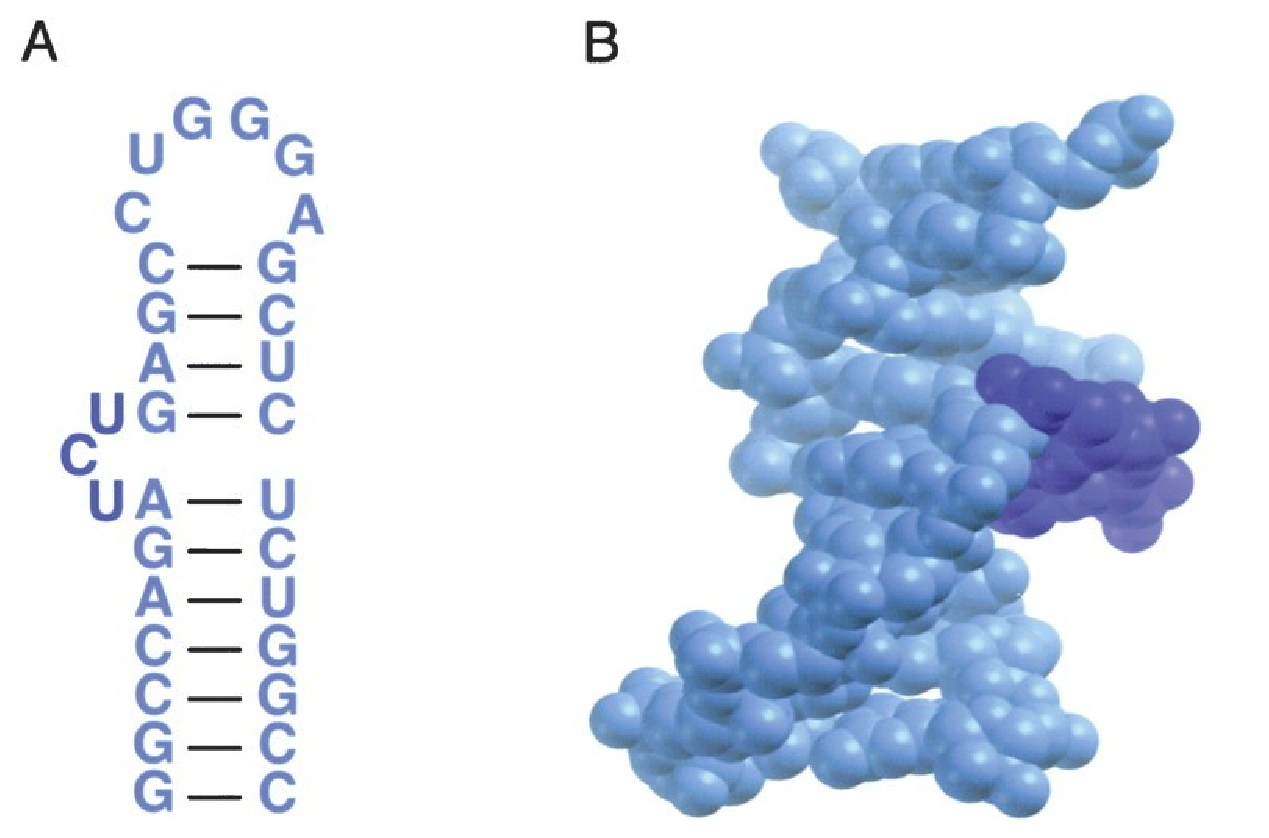
\includegraphics{RNAss}
\caption%[]
{
Estructura secundaria de un RNA (A) correspondiente a la estructura (B), tomada de \cite{Noller2004} y reproducida con permiso.
}
\label{fig:RNAss}
\end{center}
\end{figure}

La estructura secundaria de una mol\'{e}cula de RNA, sostenida por medio de 
puentes de hidr\'{o}geno (de tipo Watson-Crick y
%\htmladdnormallink{puentes de hidr\'{o}geno}{http://www.fli-leibniz.de/IMAGE\_BPDIR.html} (de tipo Watson-Crick y 
\htmladdnormallink{Hoogsteen}{http://en.wikipedia.org/wiki/Hoogsteen_base_pair}) entre nucle\'{o}tidos,
puede aproximarse a partir del conocimiento de la secuencia, aunque obviamente se pierde parte de la complejidad
del plegamiento, como sugiere la figura \ref{fig:RNAss}. Para qu\'{e} sirven este tipo de predicciones? 
Por ejemplo, para descubrir RNAs no codificantes, que a menudo tienen funciones biol\'{o}gicas importantes, 
como se discute en el art\'{i}culo de \cite{Washietl2005}.
%ste \htmladdnormallink{art\'{i}culo}{./papers/ncRNAs2005.pdf} de \citet{Washietl2005}. 
Hay muchos programas disponibles que pueden ayudarnos en este tipo de tareas, como 
\htmladdnormallink{MC-Fold | MC-Sym}{http://www.major.iric.ca/MC-Pipeline},
\htmladdnormallink{Mfold}{http://mfold.rna.albany.edu/?q=mfold},
%\htmladdnormallink{UNAFold}{http://www.bioinfo.rpi.edu/applications/hybrid/download.php},
\htmladdnormallink{Vienna}{http://www.tbi.univie.ac.at/~ivo/RNA/},
\htmladdnormallink{RNAz}{http://www.tbi.univie.ac.at/~wash/RNAz/}, 
\htmladdnormallink{infernal}{http://infernal.janelia.org/} o
\htmladdnormallink{EDeN}{http://www.bioinf.uni-freiburg.de/~costa/EDeN.tgz}, especializado en ncRNAs.

Un programa complementario, que asigna elementos de estructura secundaria dadas unas coordenadas en formato PDB, es 
\htmladdnormallink{DSSR}{http://dssr.x3dna.org}.

Aqu\'{i} nos vamos a centrar en ilustrar el algoritmo de \citet{Nussinov1978} para predecir estructura secundaria de RNA 
por medio de alineamientos, %que ya vimos de pasada en el programa de la secci\'{o}n \ref{dna2}, 
que usa una estrategia de 
\htmladdnormallink{programaci\'{o}n din\'{a}mica}{http://es.wikipedia.org/wiki/Programaci\%C3\%B3n_din\%C3\%A1mica_(inform\%C3\%A1tica)} (DP)
para maximizar el n\'{u}mero de puentes de hidr\'{o}geno que se forman dentro de la secuencia. \'{E}ste puede decirse que es
el algoritmo fundamental para resolver este problema aunque tiene algunas limitaciones. Por ejemplo, no considera la posibilidad de 
pseudonudos (\htmladdnormallink{\italics{pseudoknots}}{http://en.wikipedia.org/wiki/Pseudoknot}) ni tiene en cuenta el 
apilamiento de bases (\italics{base stacking}),
un tipo de interacci\'{o}n que favorece la estabilidad de estas estructuras, elementos que s\'{i} son proyectados en el
\htmladdnormallink{software actual}{http://en.wikipedia.org/wiki/List_of_RNA_structure_prediction_software} \citep{dotu_ivan_2014_1066354}.

El c\'{o}digo fuente que se muestra implementa este algoritmo, 
evaluando recursivamente hasta 4 situaciones en cada posici\'{o}n de la matrix DP \citep{Eddy2004b}:
\begin{itemize}
\item caso1: nuevo par de bases alineado
\item caso2: indel en un extremo, se conserva score anterior
\item caso3: indel en extremo opuesto, se conserva score
\item caso4: bifurcaci\'{o}n en base $k$ si hay distancia suficiente 
\end{itemize}

\verbatiminput{code/prog2.1.pl}

%\begin{figure}
%\begin{center} 
%\includegraphics{RNAdp}
%\caption
%{
%Recursiones y etapas de programaci\'{o}n din\'{a}mica para el estudio de la estructura secundaria de una secuencia RNA,
%tomadas de \cite{Eddy2004b}. 
%}
%\label{fig:RNAdp}
%\end{center}
%\end{figure}
%no gratuito

\begin{figure}
\begin{center} 
\includegraphics{RNAdotplot}
\caption
{
Estructura secundaria de una mol\'{e}cula de RNA y matriz (dot plot) que esquematiza sus puentes de hidr\'{o}geno.
Figura tomada de \cite{Bernhart2006} y reproducida con permiso. 
}
\label{fig:RNAdotplot}
\end{center}
\end{figure}
